\section{Evolving Neural Networks for a Flatland Agent}
\subsection{EA-parameters}
\begin{center}

\begin{tabular}{p{5cm} | r}
\textbf{Parameter} & \textbf{Value} \\
\hline
Population & 75 \\
Maximum iterations & 200 \\
Elitism & 5 \\
Tournament size & 10 \\
Tournament epsilon & 0.2 \\
Mutation percent & 0.05 \\
Crossover rate & 0.2 \\
\hline
\end{tabular}
\end{center}

To find these parameters we tried dozens of complete runs, also with different parent mate selection and adult selection mechanisms. In the end we ended up using \textbf{Tournament selection} along with \textbf{Generation Mixing} in the Evolutionary algorithm to evolve a fairly good agent to move around in the Flatland world.

\subsection{Fitness function}
During the simulation of the robot in the flatland world we count the number of food pickups, $x$ and the number of poison pickups, $y$. 
\begin{center}
	$f(x, y) = x - y$
\end{center}

This fitness function is very simple, it takes the number of foods picked up and penalizes poison pickups with subtraction from the food pickups.

\subsection{ANN design}

\begin{figure}[H]
  \centering
    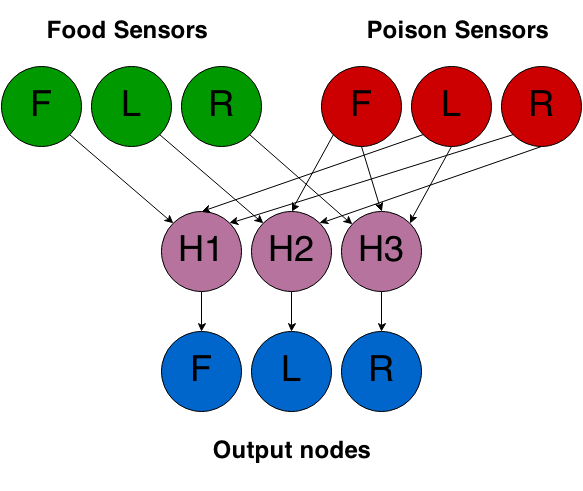
\includegraphics[width=0.5\textwidth]{img/Flatland_network}
    \caption{Artificial Neural Network for the Flatland Agent.}
\end{figure}

Three hidden nodes represents the layer between the input sensors and the output nodes. The main idea of the hidden nodes is to understand that the poison is negative and food is positive for the final outputs. The food input sensors is linked to the "same" hidden node, while the poison input sensors is linked to the "opposite" hidden node. 

The weights in this artificial neural network can have values $[-1, 1]$. Inside each neuron the Sigmoid function is used to calculate if the neuron is activated or not. The input to the Sigmoid function is the weight of each input node that is activated. The neuron will be activated if:

\begin{center}
	$\frac{1}{1 + \exp^{-x}} \geq 0.5$
\end{center}

Where x is the sum of weights times each connected neurons activation (0 or 1).

The weights is evolved from the evolutionary algorithm. The bitstring from the EA is splitted up in groups of 8 bits per weight and then converted into a number in the weight range. This is of course easy to change with parameters to have higher precision to the weights in the ANN, and we found out that 8 bits as one weight was a good number to produce good results. With $x$ bits to each weight, our network with 12 edges, the EA will have to deal with $12x$ bits.

\subsection{Differences in performance of the EA on a static \\versus a dynamic run}

TODO: Oppdatere disse grafene

\begin{figure}[H]
  \centering
    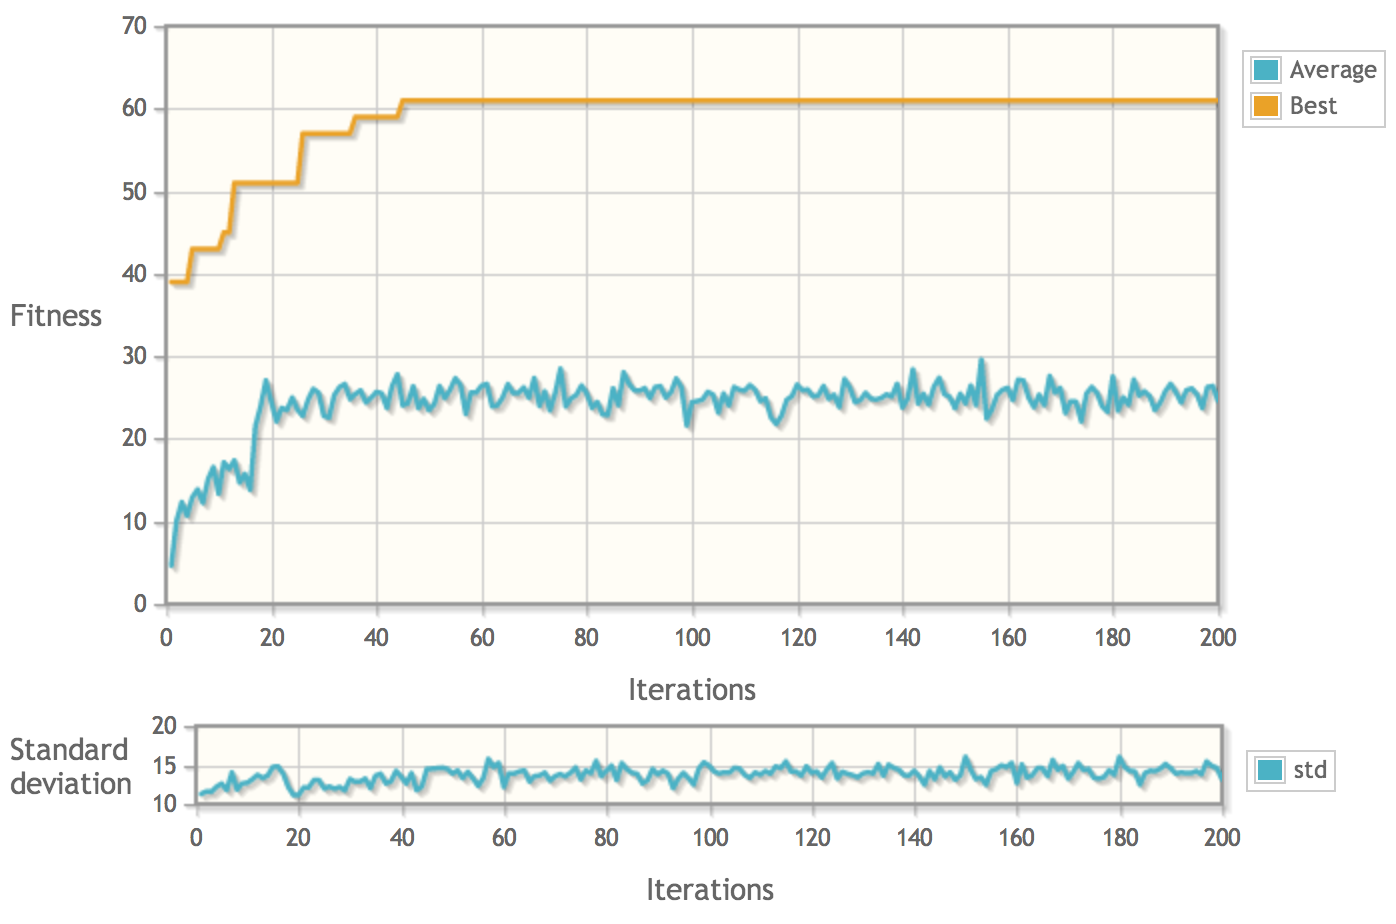
\includegraphics[width=0.8\textwidth]{img/Flatland_static}
    \caption{Fitness plot for static run}
\end{figure}

\begin{figure}[H]
  \centering
    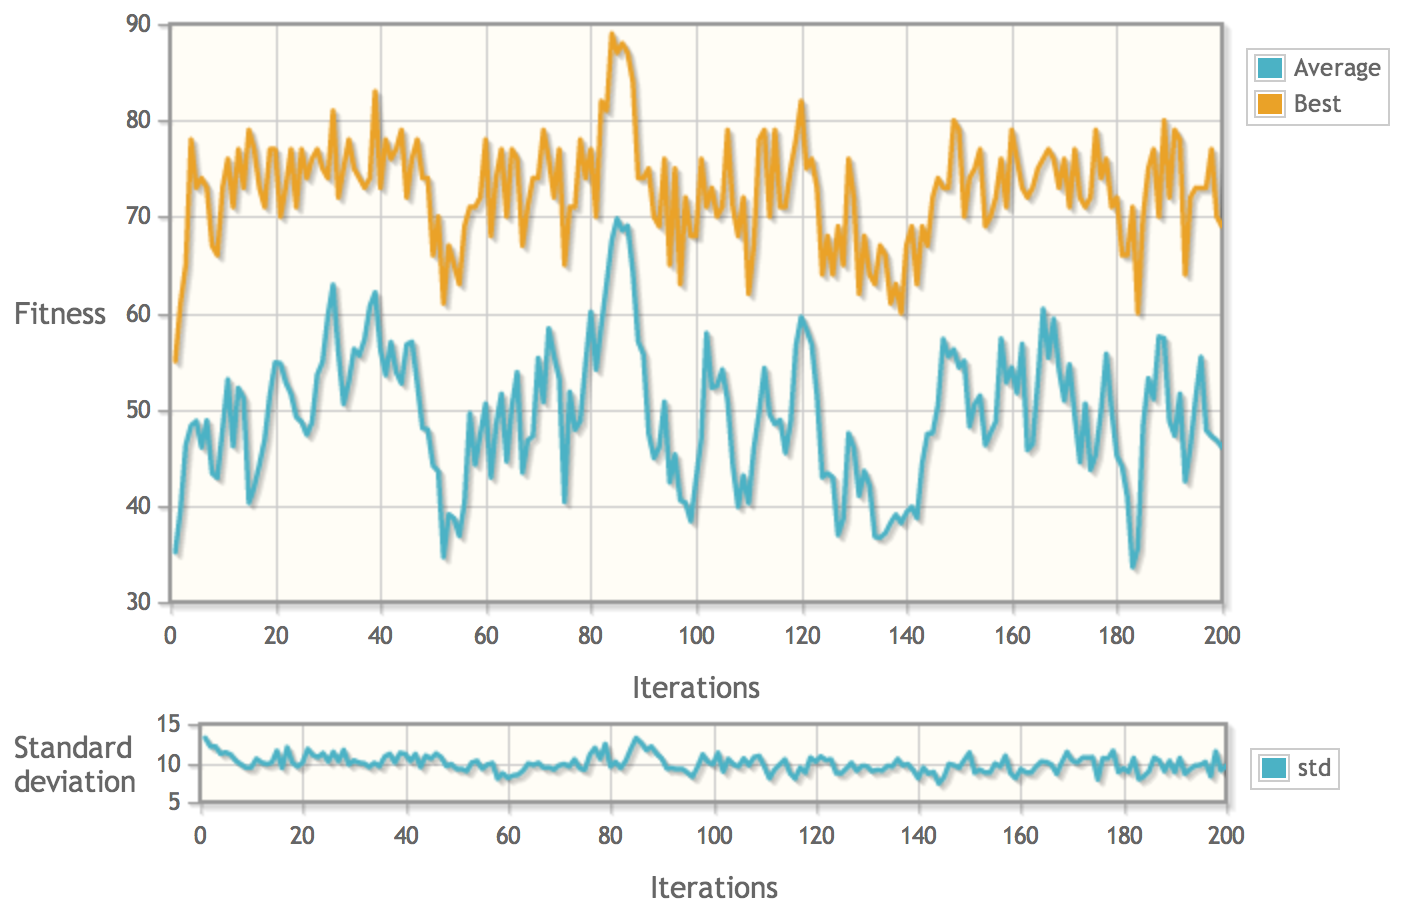
\includegraphics[width=0.8\textwidth]{img/Flatland_dynamic}
    \caption{Fitness plot for dynamic run}
\end{figure}

